\documentclass[11pt]{style/memo}

\usepackage{tikz}
    \usetikzlibrary{arrows.meta}
\usepackage{amsmath, amssymb}
\usepackage{cancel}
\usepackage{multirow}

\title{Nonlinear Coupled Physics}
\author{Kevin J. Dugan}
\date{January 6, 2020}

\begin{document}
\maketitle

\section{Introduction}
This document outlines how a nonlinear system of physics models can be formulated into
an algebraic system. The formulation will use a finite element spatial discretization and a
Newton method.

\section{Single Phyiscs Formulation}
To illustrate the process for generating this nonlinear system of equations, a 1D nonlinear, 
single-physics model will be taken; a nonlinear heat conduction model (\ref{eq:single_model}) is
chosen.

\begin{equation}
    \label{eq:single_model}
    \begin{gathered}
    -\frac{d}{dx} \left( k(T) \frac{dT}{dx} \right) = Q,     \qquad x \in [0,L] \\
    \left. \frac{dT}{dx} \right|_{x=0} = 0,                  \qquad T(L) = T_\mathrm{right},  \qquad k(T) = 0.12 + 0.75 e^{-0.05{\left(T-450 \right)}^2},
    \end{gathered}
\end{equation}
\vspace{1em}

where we will consider the domain of ${x\in[0, 40]}$, and the dirichlet temperature is
$T_\mathrm{right} = 400$.

\subsection{Residual Formulation}
This section will walk through the process of generating the discretized nonlinear residual. We pose
the problem as a root finding system

\begin{equation*}
    \mathrm{given} \ \vec{F}(\vec{U}):\mathbb{R}^n \rightarrow \mathbb{R}^n,
    \ \mathrm{find} \ \vec{U}^\ast \in \mathbb{R}^n \ \mathrm{such \ that}
    \ \vec{F}(\vec{U}^\ast) = 0.
\end{equation*}

Hence, the model in (\ref{eq:single_model}) would have the nonlinear residual

\begin{equation*}
    F(T) = -\frac{d}{dx} \left( k(T) \frac{dT}{dx} \right) - Q,
\end{equation*}

where the vector notation has been temporarily dropped because the above residual is defined in
continuous space. Spatial discretization can be achieved through a finite element formulation by
left-multiplying by a basis vector and integrating over the domain.

\begin{equation*}
    - \int_\Omega \vec{b}_i \frac{d}{dx} \left( k(T) \frac{dT}{dx} \right) - \int_\Omega \vec{b}_i Q
\end{equation*}

The first term can be simplified by using integration by parts (which can be derived from the product
rule for differentiation). The following is referred to as the \emph{weak form} of (\ref{eq:single_model}).

\begin{equation}
    \int_\Omega k(T) \frac{d\vec{b}_i}{dx} \frac{dT}{dx}
    - \left. k(T) \vec{b}_i \frac{dT}{dx} \right|_{\partial\Omega}
    -\int_\Omega \vec{b}_i Q
    \label{eq:weak_form}
\end{equation}

Since the model problem (\ref{eq:single_model}) has homogeneous Neumann boundary conditions, the
second term in the above will evaluate to zero and thus will be dropped. If non-homogeneous Neumann
conditions were present, these contributions would appear in the system assembly. To finish the
discretiztion, an approximation must be made for the solution

\begin{equation*}
    T(x) \approx \sum_j T_j b_j(x)
\end{equation*}

Substituting this approximation into the residual yields the discretized form of the residual we
will work with (\ref{eq:single_residual})

\begin{equation}
    \left[ \int_\Omega k(T) \frac{d\vec{b}_i}{dx} \frac{d\vec{b}_j^T}{dx} \right] \vec{T}
    -\int_\Omega \vec{b}_i Q
    \label{eq:single_residual}
\end{equation}

where $\vec{T}$ is a vector of the $\{T_j\}$ coefficients. Notice that the conductivity $k(T)$ is
still evaluated at the continuous approximation of $T(x)$.

\hspace{1em} The integrals over the domain are computed by suming the contributions from each cell in the
discretization. Assume the domain is covered by a set of non-overlapping cells described in 
Section~\ref{sec:basis}. Then the integral can be formulated as

\begin{equation*}
    \left[ \sum_{E\in\Omega} \int_E k(T) \frac{d\vec{b}_i}{dx} \frac{d\vec{b}_j^T}{dx} \right] \vec{T}
    - \sum_{E\in\Omega} \int_E \vec{b}_i Q
\end{equation*}

We can take advantage of a quadrature formula of integration over the cell, provided we transform
the domain cell to a reference cell. For example, the domain cell ($E$) may span ${x\in[x_i, x_{i+1}]}$,
while the reference cell ($\mathcal{E}$) may span ${\xi\in[-1,1]}$, where we define the Jacobian of the transformation
as

\begin{equation*}
    \mathcal{J} = \frac{dx}{d\xi}.
\end{equation*}

Our residual now becomes an integral over the reference cell with the proper transformations in place.
There will be some cancelations of Jacobians due to the change of variables and gradients of basis
functions.

\begin{equation*}
    \left[ \sum_{E\in\Omega} \int_\mathcal{E} k(T) 
        \left(\frac{d\vec{b}_i}{d\xi} \mathcal{J}^{-1} \right)
        \left(\frac{d\vec{b}_j^T}{d\xi} \mathcal{J}^{-1} \right) \mathcal{J} \right] \vec{T}
    - \sum_{E\in\Omega} \int_\mathcal{E} \vec{b}_i Q \mathcal{J}
\end{equation*}

where the basis functions $\vec{b}_{i,j}$ are now defined on the reference cell. Now that the integrals
are over the reference cell, a quadrature formula may now be used.

\begin{equation}
    \vec{F}_i(\vec{T}) = 
    \left[ \sum_{E\in\Omega} \sum_q w_q k(T_q) 
        \left. \frac{d\vec{b}_i}{d\xi} \right|_{\xi_q}
        \left. \frac{d\vec{b}_j^T}{d\xi} \right|_{\xi_q} \mathcal{J}^{-1} \right] \vec{T}
    - \sum_{E\in\Omega} \sum_q w_q \vec{b}_i(\xi_q) Q(x(\xi_q)) \mathcal{J}
\end{equation}

\subsection{Jacobian Formulation}
The Jacobian used in Newton's method is a matrix of first derivatives of the nonlinear residual

\begin{equation*}
    \mathbf{J}_{ij}(\vec{U}) = \frac{\partial \vec{F}_i(\vec{U})}{\partial \vec{U}_j}
\end{equation*}

The Jacobian for a discretized nonlinear residual generated from a finite element method is
derived in a straight-forward manner in this section. We begin by using the above formula with
(\ref{eq:single_residual}) to start the derivation

\begin{equation*}
    \mathbf{J}_{ij} = \frac{\partial}{\partial T_j} \left[ 
        \int_\Omega k(T) \frac{d\vec{b}_i}{dx} \left(\sum_k \frac{d\vec{b}_k^T}{dx} T_k \right) \right]
    - \cancelto{0}{ \frac{\partial}{\partial T_j} \int_\Omega \vec{b}_i Q }
\end{equation*}

Note that the product of the coefficient vector and the shape function gradient is explicitly written
as a sum to not confuse the residual construction with taking the derivative with respect to the
$j$-th coefficient. Pulling the derivative into the integrand and using the product rule and chain
rule

\begin{equation}
    \label{eq:single_jacobian}
    \int_\Omega \frac{d\vec{b}_i}{dx} \left( \frac{dk}{dT}\frac{\partial T}{\partial T_j}\right) \left(\sum_k \frac{d\vec{b}_k^T}{dx} T_k \right)
    + \int_\Omega k(T) \frac{d\vec{b}_i}{dx} \frac{d\vec{b}_j^T}{dx}
\end{equation}

In the second term of the product rule, we use the solution gradient approximation

\begin{equation*}
    \frac{dT}{dx} \approx \sum_k \frac{db_k(x)}{dx}T_k
\end{equation*}

\begin{equation*}
    \frac{\partial}{\partial T_j} \left( \sum_k \frac{db_k(x)}{dx}T_k \right) = \frac{db_j(x)}{dx}
    \cancelto{1}{\frac{dT_j}{dT_j} }
\end{equation*}

Similarly the $\frac{\partial T}{\partial T_j}$ term can be reduced to $\vec{b}_j^T$ using a similar formulation
as above. Again, a quadrature formula over the set of cells in the domain can be used to generate the final
assembly formulation

\begin{equation}
    \mathbf{J}_{ij}(\vec{T}) = \sum_{E\in\Omega}\sum_q w_q \left[
        \left. \frac{d\vec{b}_i}{d\xi} \vec{b}_j^T \frac{dT}{d\xi} \right|_{\xi_q} \frac{dk}{dT}
    + k(T_q) \left. \frac{d\vec{b}_i}{d\xi} \frac{d\vec{b}_j^T}{d\xi} \right|_{\xi_q} \right] \mathcal{J}^{-1}
\end{equation}

where $\frac{dT}{dx}$ is the finite element approximation gradient evaluated at $\xi_q$, i.e. $\sum_k \frac{db_k(\xi_q)}{dx}T_k$. With these
formulations, the solution can be found using Newton's method where the solution is updated as follows

\begin{equation}
\begin{gathered}
    \delta\vec{U} = - \mathbf{J}{(\vec{U}^{n})}^{-1}\vec{F}(\vec{U}^{n}) \\
    \vec{U}^{n+1} = \vec{U}^{n} + \delta\vec{U}.
\end{gathered}
\end{equation}

\subsection{Boundary  Conditions}\label{sec:bcs}
In the context of finite element discretizations, two categories of boundary conditions can be found.
The first is \emph{Natural} --- these appear naturally in the weak formulation (\ref{eq:weak_form}).
The other is \emph{Dirichlet} --- these are imposed conditions once the global system has been
assembled.

\hspace{1em} To impose Natrual boundary conditions, boundary elements are identified in the system assembly process
and contributions from corresponding boundary terms are added to the global system with other weak
form terms.

\hspace{1em} Dirichlet conditions are imposed as a final step once the global system has been formed. For a linear
system assembly, the system matrix row corresponding to the dirichlet node is zeroed while a one is
placed on the diagonal element. The corresponding right hand side element is replaced with the dirichlet
value. For example, if $x_d$ is a dirichlet node with value $D$

\begin{equation*}
\begin{bmatrix}
a_{0,0} & \cdots & a_{0,d-1} & a_{0,d} & a_{0,d+1} & \cdots & a_{0,N} \\
\vdots  & \ddots & \vdots    & \vdots  & \vdots    & \ddots & \vdots  \\
0       & \cdots & 0         & 1       & 0         & \cdots & 0       \\
\vdots  & \ddots & \vdots    & \vdots  & \vdots    & \ddots & \vdots  \\
a_{N,0} & \cdots & a_{N,d-1} & a_{N,d} & a_{N,d+1} & \cdots & a_{N,N} \\
\end{bmatrix}
\begin{bmatrix}
    x_0 \\ \vdots \\ x_d \\ \vdots \\ x_N
\end{bmatrix} = 
\begin{bmatrix}
    b_0 \\ \vdots \\ D \\ \vdots \\ b_N
\end{bmatrix}
\end{equation*}

This process is repeated for all dirichelt nodes in the system. A typical desire is to maintain a
symmetric matrix, which is achieved by distributing $a_{i,d}*D$ into the right hand side. Thus, the
entries become $b_i - a_{i,d}*D$, excluding the $b_d$ entry.

\hspace{1em} A similar procedure is followed for nonlinear systems except that the nonlinear residual
is constructed as $F_d = U_d - D$. The Jacobian matrix is modified identically to the matrix $A$
above.

\subsection{Discretization and Basis Functions}\label{sec:basis}
In this section I discuss the spatial discretization and useful basis functions which can be used. We
assume that the domain is discretized using a non-overlapping set of $N$ cells $\Omega$. In a 1D
domain, we can structure the discretization as

\begin{equation*}
    \Omega = \begin{bmatrix}
        x_0 & x_1 \\
        x_1 & x_2 \\
        \vdots & \vdots \\
        x_{N-1} & x_N
    \end{bmatrix}
\end{equation*}

In reality, this is achieved by using a list of spatial points and a connectivity matrix but the
above formulation will suffice for this discussion.

\hspace{1em} A set of basis functions must be chosen overwhich to expand the solution. There are many
choices available for such basis function. A good starting point is to use the Lagrange polynomials
over the domain $\xi \in [-1,1]$. The first few sets of basis functions from this space is shown in
Table~\ref{tab:lagrange}.

\begin{table}
\centering
\caption{Lagrange polynomial definitions}
\begin{tabular}{@{}ccc@{}}\toprule
\textbf{Order} & \textbf{Polynomial}\\ \midrule 
\multirow{2}{*}{1} & $\frac{1}{2}(1-\xi)$ \vspace{0.5em} \\
                   & $\frac{1}{2}(1+\xi)$ \vspace{0.5em} \\ \midrule
\multirow{3}{*}{2} & $-\frac{1}{2}\xi(1-\xi)$ \vspace{0.5em} \\
                   & $(1-\xi)(1+\xi)$ \vspace{0.5em} \\
                   & $\frac{1}{2}\xi(1+\xi)$ \vspace{0.5em} \\ \midrule
\multirow{4}{*}{3} & $-\frac{1}{16}(1-\xi)(1+3\xi)(1-3\xi)$ \vspace{0.5em} \\
                   & $-\frac{1}{16}(1+\xi)(1+3\xi)(1-3\xi)$ \vspace{0.5em} \\
                   & $\frac{9}{16}(1+\xi)(1-\xi)(1-3\xi)$ \vspace{0.5em} \\
                   & $\frac{9}{16}(1+\xi)(1-\xi)(1+3\xi)$ \vspace{0.5em} \\
\bottomrule
\end{tabular}\label{tab:lagrange}
\end{table}

\hspace{1em}Instead of taking strictly the Lagrange polynomials, we may opt to build a hierarchical set of polynomials.
This is acheived by taking the linear Lagrange functions and appending one function from the higher
order Lagrange sets; specifically we choose one of the functions which vanish at the boundary to
preserve continuity. An example of this hierarchical set is defined on the reference element ($\mathcal{E}$).

\begin{equation}
    \label{eq:basis_fn}
    \vec{b}(\xi) = \frac{1}{2} \begin{bmatrix}
        1-\xi \\
        1+\xi \\
        2 \left( 1-\xi^2 \right) \\
        \frac{9}{8} (1 - 3\xi - \xi^2 + 3 \xi^3)
    \end{bmatrix}
\end{equation}

which are shown in Figure~\ref{fig:basis}.

\begin{figure}[h!]
    \centering
    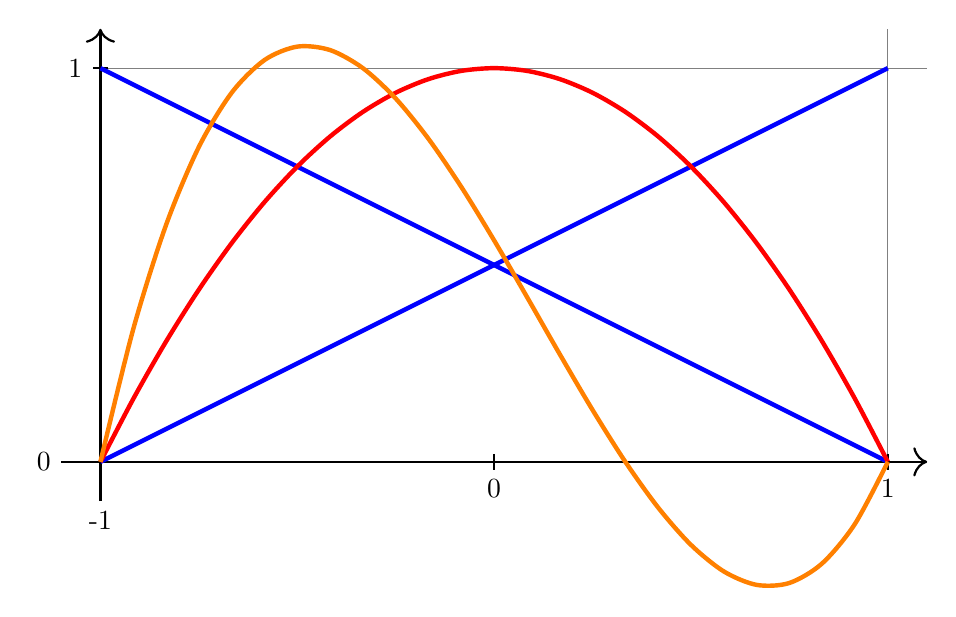
\begin{tikzpicture}
        \draw[gray] (-5,5) -- (5.5,5);
        \draw[gray] (5,0) -- (5,5.5);
        \draw[thick, -{>[scale=1.5]}] (-5.5,0) node[anchor=east] {0} -- (5.5,0);
        \draw[thick] (0,0.1) -- (0,-0.1) node[anchor=north] {0};
        \draw[thick] (5,0.1) -- (5,-0.1) node[anchor=north] {1};
        \draw[thick, -{>[scale=1.5]}] (-5,-0.5) node[anchor=north] {-1} -- (-5,5.5);
        \draw[thick] (-4.9,5) -- (-5.1,5) node[anchor=east] {1};

        \draw[ultra thick, domain=-5:5, smooth, variable=\x, blue] plot ({\x}, {5.0*0.5*(1.0+\x/5.0)});
        \draw[ultra thick, domain=-5:5, smooth, variable=\x, blue] plot ({\x}, {5.0*0.5*(1.0-\x/5.0)});
        \draw[ultra thick, domain=-5:5, smooth, variable=\x, red] plot ({\x}, {5.0*(1.0-(\x/5.0)*(\x/5.0))});
        \draw[ultra thick, domain=-5:5, smooth, variable=\x, orange] plot ({\x}, {5.0*0.5625*(1.0-3.0*(\x/5.0)-(\x/5.0)*(\x/5.0)+3.0*(\x/5.0)*(\x/5.0)*(\x/5.0))});
    \end{tikzpicture}
    \caption{Hierarchical Lagrangian basis functions up to order 3}\label{fig:basis}
\end{figure}

In this setup, the transformation Jacobian $\mathcal{J}$ for cell $i$ is defined as

\begin{equation*}
    \mathcal{J}_i = \frac{dx}{d\xi} = \frac{x_i - x_{i-1}}{2} \qquad i = 1, 2, \dots, N
\end{equation*}

\newpage
\underline{Optional Extensions}
\begin{itemize}
    \item 2D basis functions and generalized residual/Jacobian
    \item Coupled physics section (heat generation dependent on other physics component)
\end{itemize}

\nocite{segerlind-1984, zienkiewicz-2005, guermond-2000}
\bibliographystyle{unsrt}
\bibliography{references}

\end{document}
